\chapter{DTP and VTP}\label{dtp-and-vtp}

DTP (Dynamic Trunking Protocol)

\begin{itemize}
\tightlist
\item
  Protocol that allows SWITCHES to negotiate the status of their
  SWITCHPORTS, without manual configuration, to be:

  \begin{itemize}
  \tightlist
  \item
    ACCESS PORTS
  \item
    TRUNK PORTS
  \end{itemize}
\item
  DTP is ENABLED by default on all Cisco SWITCH interfaces
\end{itemize}

We've been manually configuring SWITCHPORTS using :

\begin{itemize}
\tightlist
\item
  ``switchport mode access''
\item
  ``switchport mode trunk''
\end{itemize}

\begin{tipbox}

`show interfaces switchport' will show you a switchport's settings.

\end{tipbox}

For security purposes, \textbf{manual configuration} is recommended. DTP
should be disabled on ALL SWITCHPORTS

\begin{figure}
\centering
\pandocbounded{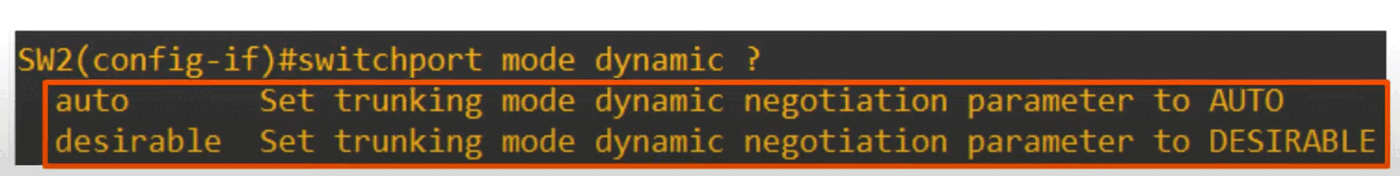
\includegraphics[keepaspectratio,alt={image}]{images/20-dtp-vtp/img-001.png}}
\end{figure}

\section{Dynamic Desirable}\label{dynamic-desirable}

\begin{itemize}
\tightlist
\item
  This MODE will actively try to form a TRUNK with other Cisco SWITCHES.
\item
  Will form a TRUNK if connected to another SWITCHPORT in the following
  modes:

  \begin{itemize}
  \tightlist
  \item
    ``switchport mode trunk''
  \item
    ``switchport mode dynamic desirable''
  \item
    ``switchport mode dynamic auto''
  \end{itemize}
\end{itemize}

HOWEVER \ldots{} if the other interface is set to ``static access''
(ACCESS mode), it will NOT form a TRUNK, it will be an ACCESS PORT

\section{Dynamic Auto}\label{dynamic-auto}

\begin{itemize}
\tightlist
\item
  This MODE will NOT actively try to form a TRUNK with other Cisco
  SWITCHES
\item
  Will form a TRUNK if connected SWTICH is actively trying to form a
  TRUNK.
\item
  It will form a TRUNK with a SWITCHPORT in the following modes:

  \begin{itemize}
  \tightlist
  \item
    ``switchport mode trunk''
  \item
    ``switchport mode dynamic desirable''
  \end{itemize}
\end{itemize}

TRUNK to ACCESS connection will operate in a \textbf{Mismatched Mode}.

This configuration does NOT work and SHOULD result in an error. Traffic
will NOT work.

\section{Table Showing the Different Modes and Compatibility in Forming
a
Trunk}\label{table-showing-the-different-modes-and-compatibility-in-forming-a-trunk}

\begin{figure}
\centering
\pandocbounded{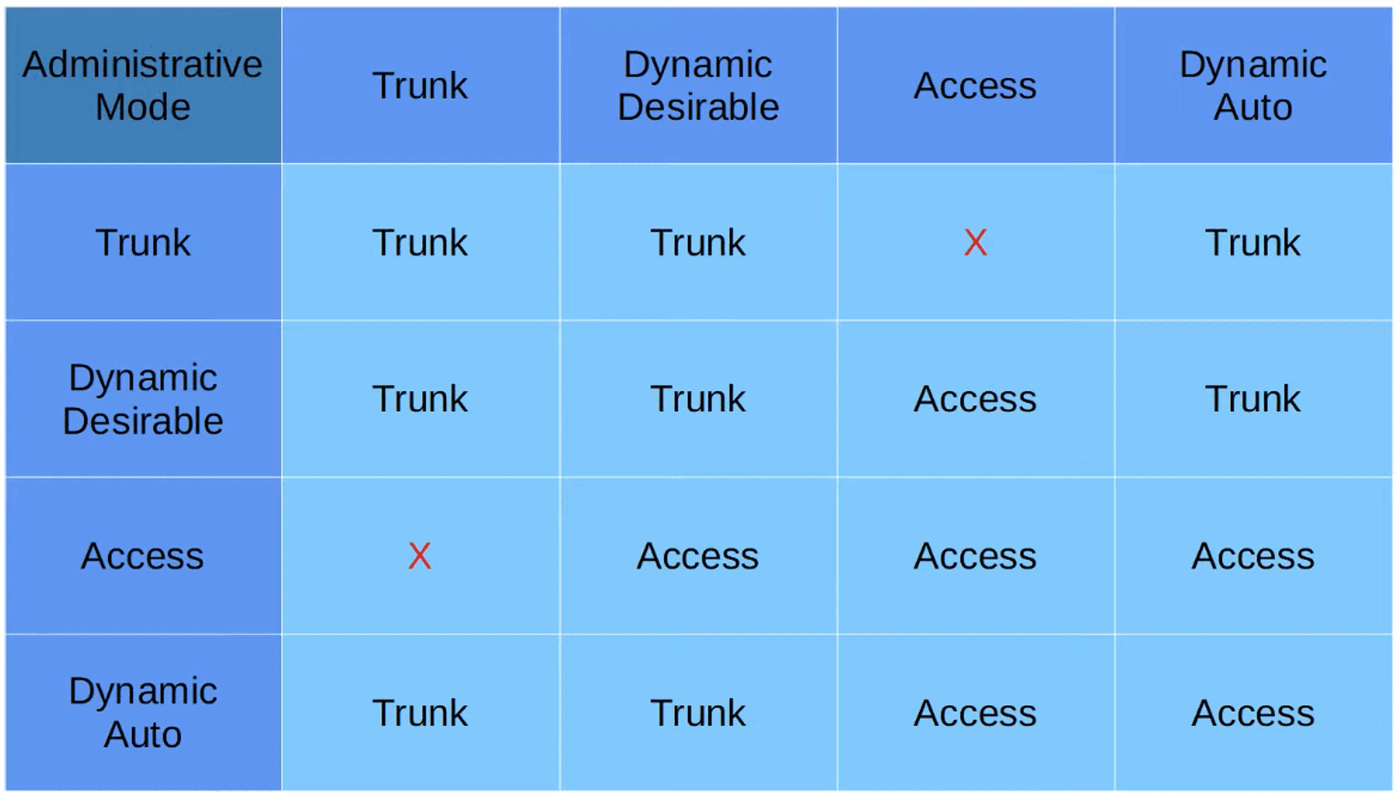
\includegraphics[keepaspectratio,alt={image}]{images/20-dtp-vtp/img-002.png}}
\end{figure}

DTP will NOT form a TRUNK with:

a ROUTER

a PC

etcetera \ldots{}

The SWITCHPORT will be in ACCESS Mode only!

\section{Old Switches}\label{old-switches}

\begin{itemize}
\tightlist
\item
  ``switchport mode dynamic desirable'' = Default administrative mode.
\end{itemize}

\section{Newer Switches}\label{newer-switches}

\begin{itemize}
\tightlist
\item
  ``switchport mode dynamic auto'' = Default administrative mode.
\end{itemize}

\section{How to Disable DTP Negotiation on an
Interface}\label{how-to-disable-dtp-negotiation-on-an-interface}

\begin{itemize}
\tightlist
\item
  ``switchport nonegotiate''
\item
  ``switchport mode access''
\end{itemize}

It is a security recommendation to disable DTP on all SWITCHPORTS and
manually configure them as ACCESS or TRUNK ports.

\section{Encapsulation}\label{encapsulation}

SWITCHES that support both:

\begin{itemize}
\tightlist
\item
  802.1Q
\item
  ISL
\end{itemize}

TRUNK encapsulation can use DTP to negotiate the encapsulation they will
use.

\begin{itemize}
\tightlist
\item
  Negotiation is Enabled by default
\end{itemize}

\begin{tipbox}

`switchport trunk encapsulation negotiate'

\end{tipbox}

\begin{itemize}
\tightlist
\item
  ISL is favored over 802.1Q

  \begin{itemize}
  \tightlist
  \item
    If BOTH SWITCHES support ISL, ISL will be selected.
  \end{itemize}
\item
  DTP frames are sent in:

  \begin{itemize}
  \tightlist
  \item
    VLAN1 when using ISL
  \item
    Native VLAN when using 802.1Q (the default native VLAN is VLAN1,
    however)
  \end{itemize}
\end{itemize}

VTP (VLAN Trunking Protocol)

In Privileged EXEC mode:

\begin{tipbox}

\#show vtp status

\end{tipbox}

\begin{itemize}
\item
  Protocol for configuring VLANs on a Central SWITCH

  \begin{itemize}
  \tightlist
  \item
    A SERVER that other SWITCHES synch. to (auto configuring by
    connection)
  \end{itemize}
\item
  Other switches (VTP CLIENTS) will synchronize their VLAN database to
  the SERVER
\item
  Designed for large networks with many VLANs (reduces manual
  configuration)
\item
  RARELY used. Recommended you DO NOT USE it
\item
  There are THREE VTP Versions :

  \begin{itemize}
  \tightlist
  \item
    v1

    \begin{itemize}
    \tightlist
    \item
      Does NOT supports Extended VLAN Range 1006-4094
    \end{itemize}
  \item
    v2

    \begin{itemize}
    \tightlist
    \item
      Does NOT supports Extended VLAN Range 1006-4094
    \item
      Supports Token Ring VLANs ; otherwise similar to V1
    \end{itemize}
  \item
    v3

    \begin{itemize}
    \tightlist
    \item
      Supports Extended VLAN Range 1006-4094
    \item
      CLIENTS store VLAN dBase in NVRAM
    \end{itemize}
  \end{itemize}
\item
  There are \textbf{THREE VTP modes}:

  \begin{itemize}
  \tightlist
  \item
    SERVER
  \item
    CLIENT
  \item
    TRANSPARENT
  \end{itemize}
\item
  Cisco SWITCHES operate in VTP SERVER mode, by default
\end{itemize}

\begin{figure}
\centering
\pandocbounded{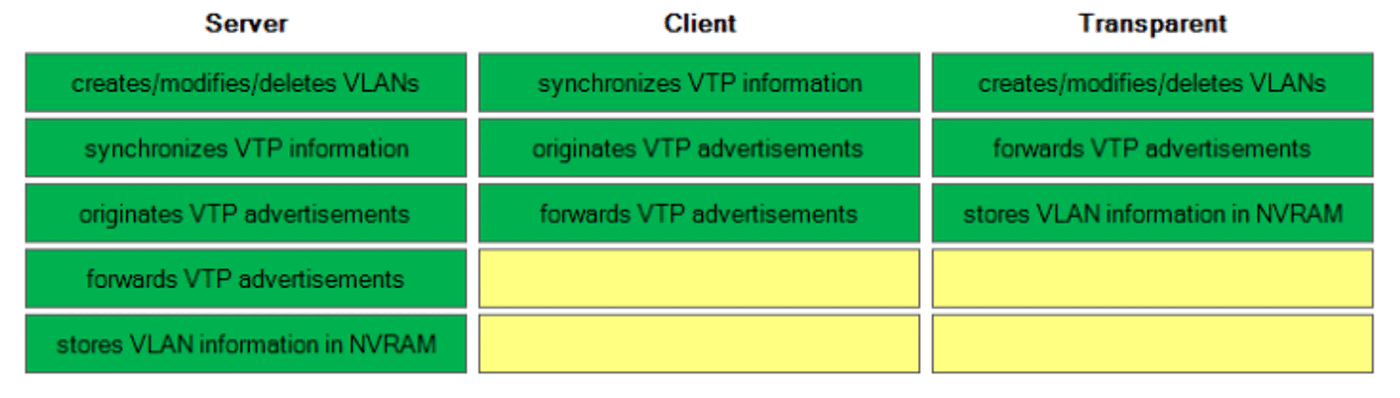
\includegraphics[keepaspectratio,alt={image}]{images/20-dtp-vtp/img-003.png}}
\end{figure}

\section{VTP Servers}\label{vtp-servers}

\begin{itemize}
\tightlist
\item
  Can ADD / MODIFY / DELETE VLANs
\item
  Store the VLAN dBase in NVRAM
\item
  Increase Revision Number every time VLAN is Added / Modified / Deleted
\item
  Advertises \textbf{Latest Version} of VLAN dBase on TRUNK interfaces.
\item
  VTP CLIENTS synchronize their VLAN dBase to it
\item
  \textbf{VTP SERVERS also function as VTP CLIENTS}

  \begin{itemize}
  \tightlist
  \item
    \textbf{THEREFORE, a VTP SERVER will synchronize to another VTP
    SERVER with a higher Revision Number}
  \end{itemize}
\end{itemize}

\begin{warnbox}

One danger of VTP: Connecting an old SWITCH with higher Revision Number
to network (and if the VTP Domain Name matches), all SWITCHES in Domain
will synchronize their VLAN dBase to SWITCH

\end{warnbox}

\section{VTP Clients}\label{vtp-clients}

\begin{tipbox}

(config)\# vtp mode client

\end{tipbox}

\begin{itemize}
\tightlist
\item
  Cannot Add / Modify / Delete VLANs
\item
  Does NOT store the VLAN database in NVRAM

  \begin{itemize}
  \tightlist
  \item
    \textbf{VTP v3 CLIENTS DO}
  \end{itemize}
\item
  Will synchronize their VLAN dBase to the SERVER with the highest
  version number in their VTP Domain
\item
  Advertise their VLAN dBase and forward VTP Advertisements to other
  CLIENTS over TRUNK Ports
\end{itemize}

\section{VTP Transparent Mode}\label{vtp-transparent-mode}

\begin{tipbox}

(config)\# vtp mode transparent

\end{tipbox}

\begin{itemize}
\tightlist
\item
  Does NOT participate in VTP Domain (does NOT sync VLAN database)
\item
  Maintains own VLAN dBase in NVRAM.
\item
  Can Add / Modify / Delete VLANs
\item
  Won't Advertise to other SWITCHES
\item
  Will forward VTP advertisements to SWITCHES in the same Domain as it.
\end{itemize}

\section{VTP Domains}\label{vtp-domains}

If a SWITCH with no VTP Domain (Domain NULL) receives a VTP
advertisement with a VTP Domain name, it will automatically join that
VTP Domain

If a SWITCH receives a VTP advertisement in the same VTP domain with a
higher revision number, it will update it's VLAN database to match

\section{Revision Numbers}\label{revision-numbers}

There are TWO ways to RESET a REVISION NUMBER to 0:

\begin{itemize}
\tightlist
\item
  Change VTP Domain to an unused Domain
\item
  Change VTP mode to TRANSPARENT
\end{itemize}

\section{VTP Version Number}\label{vtp-version-number}

\begin{tipbox}

(config)\#vtp version

\end{tipbox}

Changing the Version \# will force sync/update all connected SWITCHES to
the latest Version \#
